% mnras_template.tex 
%
% LaTeX template for creating an MNRAS paper
%
% v3.0 released 14 May 2015
% (version numbers match those of mnras.cls)
%
% Copyright (C) Royal Astronomical Society 2015
% Authors:
% Keith T. Smith (Royal Astronomical Society)

% Change log
%
% v3.0 May 2015
%    Renamed to match the new package name
%    Version number matches mnras.cls
%    A few minor tweaks to wording
% v1.0 September 2013
%    Beta testing only - never publicly released
%    First version: a simple (ish) template for creating an MNRAS paper

%%%%%%%%%%%%%%%%%%%%%%%%%%%%%%%%%%%%%%%%%%%%%%%%%%
% Basic setup. Most papers should leave these options alone.
\documentclass[fleqn,usenatbib]{mnras}

% MNRAS is set in Times font. If you don't have this installed (most LaTeX
% installations will be fine) or prefer the old Computer Modern fonts, comment
% out the following line
\usepackage{amssymb}
\usepackage{newtxtext,newtxmath}
% Depending on your LaTeX fonts installation, you might get better results with one of these:
%\usepackage{mathptmx}
%\usepackage{txfonts}

% Use vector fonts, so it zooms properly in on-screen viewing software
% Don't change these lines unless you know what you are doing
\usepackage[T1]{fontenc}

% Allow "Thomas van Noord" and "Simon de Laguarde" and alike to be sorted by "N" and "L" etc. in the bibliography.
% Write the name in the bibliography as "\VAN{Noord}{Van}{van} Noord, Thomas"
\DeclareRobustCommand{\VAN}[3]{#2}
\let\VANthebibliography\thebibliography
\def\thebibliography{\DeclareRobustCommand{\VAN}[3]{##3}\VANthebibliography}

%%%%% AUTHORS - PLACE YOUR OWN PACKAGES HERE %%%%%
% Only include extra packages if you really need them. Common packages are:
\usepackage{multirow}

\usepackage{graphicx}	% Including figure files
\usepackage{amsmath}	% Advanced maths commands

% \usepackage{newtxtext,newtxmath}
\usepackage{pict2e}
% \usepackage[greek,english]{babel}
\usepackage[T1]{fontenc}
\usepackage{tikz}
\usepackage{pgfplots}
\usetikzlibrary{decorations.pathreplacing,calligraphy,patterns}
% \usepackage{../../Papers/JML}
%%%%% copying the contents of the Jack Markup Library here for transport
	\usepackage{environ}
	\renewcommand{\d}{\mathrm d}
	\newcommand{\eref}[1]{Eq. \eqref{#1}}
	\renewcommand{\div}[2]{\frac{\d #1}{\d #2} }
	\newcommand{\pdiv}[2]{\frac{\partial #1}{\partial #2}}
	\def\LLR
	{
		~~\Longleftrightarrow~~
	}
	\def\LR
	{
		~~~\Longrightarrow~~~
	}

	\NewEnviron{spalign}
	{
		\begin{align}
			\begin{split}
				\BODY
			\end{split}
		\end{align}
	}


%%%% continuing on from here
\bibliographystyle{apalike}
% \citestyle{acmnumeric}
\title[GenCHORD]{Extremely Low Coverage Genomic Rearrangement Analysis with \codename{}}


\author[Fraser-Govil et. al.]{
Jack Fraser-Govil,$^{1}$\thanks{E-mail: jf20@sanger.ac.uk}
Ronnie Crawford,$^{1}$
Max Stammnitz,
Elizabeth Murchison,$^{2}$
Zemin Ning, $^{1}$
\\
% List of institutions
$^{1}$Wellcome Sanger Institute, Hinxton, UK\\
$^{2}$University of Cambridge, Cambridge, UK\\
}


\def\commentVisible{1}

\newcommand\comment[1]
{
	{
		\if\commentVisible1
			\color{red!70!black}
		\else
			\color{black}
		\fi

		#1
	}
}
\def\codename{\textit{GenCHORD}}


\begin{document}
\label{firstpage}
\pagerange{\pageref{firstpage}--\pageref{lastpage}}
\maketitle

	% \label{firstpage}
	
	\begin{abstract}
		We present \codename{}, a specialised step-detection algorithm suitable for detecting large-scale copy number variations from the coverage data of a sequenced, aligned genome. This algorithm is specifically tuned for detecting Structural Variations which arise during chromothripsis-induced cancer, and so permits a high degree of data reduction, whilst preserving pertinent features for cancer classification. We describe the underlying statistical and algorithmic model, demonstrate the ability of the to preserve, compress and encode information such that a simple Machine Learning model can classify and identify subtypes of Devil Facial Tumour Disease, a cancer affecting \textit{Sarcophilus harrisii}, the Tasmanian Devil, and discuss how this tool may be used in future.   
	\end{abstract}

	\section{Introduction}
		\comment{This intro (\& abstract) is currently identical to the original paper. Will rewrite at a later date to avoid self-plagiarism!}

		{The term} Genomic Rearrangements refer to large-scale Structural Variations (SVs) amongst individual genomes; including large-scale deletion, insertion, duplication and translocation of megabase-length sequences of DNA,  and often lead to genetic disorders (when present in the germ cells), or cancer (when arising from somatic mutations). When a Genomically Rearranged sample is sequenced and aligned against a reference the true sequence's novel adjacencies can be obscured, especially when the size of the rearranged regions are significantly larger than the read length. This is because the majority of  reads will still align to the reference despite the fact that their spatial location within the genome has been altered: only those reads which bridge the unusual adjacencies contain the information that a rearrangement has occurred.

		Reconstructing these rearrangements requires complex analysis, such as a haplotype phased-assembly , which is not only computationally costly, but requires the DNA be sequenced to a very high coverage, as well techniques such as Hi-C \citep{Ijaz2024}. We should like to be able to identify, analyse and classify the presence of genomic rearrangements in a simpler fashion.  

		To do this, we leverage the knowledge that chromothripsis-induced rearrangements are often associated with highly variable copy-number variations \citep{Ijaz2024,Chromo2011}. Where portions of the genome have been duplicated or deleted (generically termed 'gains' and 'losses'), the erroneous alignment leads to variations in the base-coverage reported by the alignment tool, as demonstrated in Figure \ref{Fig:Diagram}. {The locations of regions which have undergone gains and losses corresponds strongly to the edges of the regions which have been rearranged.}

		Many tools to analyse the copy-number variations exist, however in this work we modify our existing tool, \textbf{Gen}ome \textbf{C}overage \textbf{H}armonic \textbf{O}ptimiser, \textbf{R}educer and \textbf{D}enoiser (\codename{}), a novel tool tailored for this problem which leverages the power of a Bayesian hypothesis testing to infer a statistically robust denoised copy-number analysis, which is suitable for encoding into a Neural Network, and hence permit accurate detection, analysis, and classification of the genomic rearrangement.

		\begin{figure}
			\begin{center}
				\resizebox{!}{6cm}{ 
				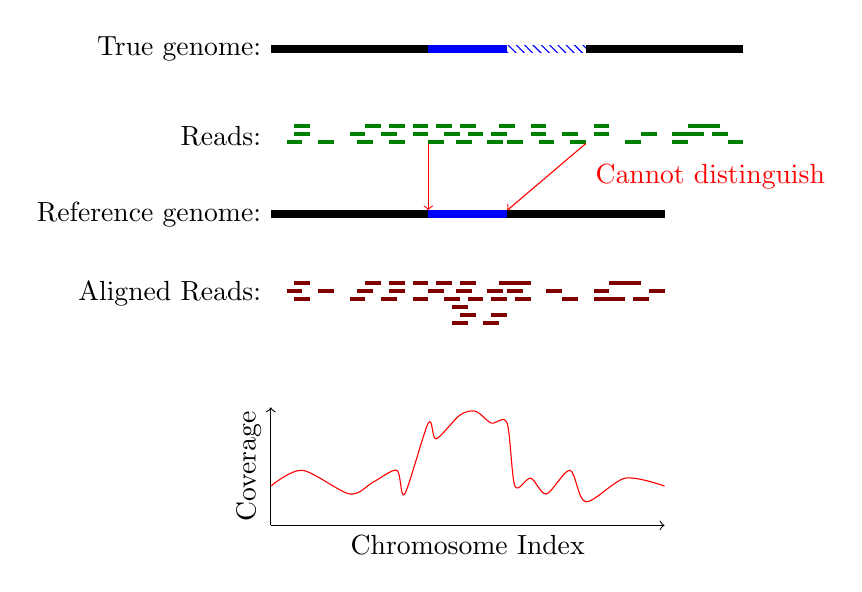
\begin{tikzpicture}
					\node[anchor=east] at (0,0.05) {True genome:};
					\fill (0,0) rectangle (2,0.1);
					\fill[blue] (2,0) rectangle (3,0.1);
					\fill[blue,pattern=north west lines, pattern color=blue] (3,0) rectangle (4,0.1);
					\fill (4,0) rectangle (6,0.1);

					\def\readheight{-1}
					\node[anchor=east] at (0,{\readheight-0.05}) {Reads:};

					\foreach[count=\i] \x in {0.3,1,1.4,1.8,2.2,2.5,2.8,3.3,3.7,4.1,4.7,5.1,5.3,5.6}
					{
						\fill[green!50!black] (\x,\readheight) rectangle ({\x+0.2},{\readheight -0.05});
					}
					\foreach[count=\i] \x in {0.2,0.6,1.1,1.5,2,2.35,2.75,3,3.4,3.8,4.5,5.1,5.8}
					{
						\fill[green!50!black] (\x,{\readheight-0.1}) rectangle ({\x+0.2},{\readheight -0.15});
					}
					\foreach[count=\i] \x in {0.3,1.2,1.5,1.8,2.1,2.4,2.9,3.3,4.1,5.3,5.5}
					{
						\fill[green!50!black] (\x,{\readheight+0.1}) rectangle ({\x+0.2},{\readheight +0.05});
					}
					\def\refheight{-2}
					\draw[->,red] (2,\readheight-0.15)--(2,\refheight);
					\draw[->,red] (4,\readheight-0.15)--(3,\refheight);
					\node[anchor=west,red] at (4,{(\refheight+\readheight-0.15)/2}) {Cannot distinguish};
					\node[anchor=east] at (0,{\refheight -0.05}) {Reference genome:};
					\fill (0,\refheight) rectangle (2,{\refheight -0.1});
					\fill[blue] (2,\refheight) rectangle (3,{\refheight -0.1});
					\fill (3,\refheight) rectangle (5,{\refheight -0.1});

					\def\areadheight{-3}
					\node[anchor=east] at (0,{\areadheight-0.05}) {Aligned Reads:};

					\foreach[count=\i] \x in {0.3,1,1.4,1.8,2.2,2.5,2.8,3.3,3.7,4.1,4.7,5.1,5.3,5.6}
					{
						\def\xoffset{0}
						\def\yoffset{0}
						\newdimen\pos
						\pos = \x cm
						\ifdim \pos > 3cm
							\def\xoffset{1}
							\ifdim \pos < 4cm
								\def\yoffset{0.3}
							\fi
						\fi
						\fill[red!50!black] ({\x-\xoffset},{\areadheight -\yoffset-0.1}) rectangle ({\x-\xoffset+0.2},{\areadheight -\yoffset-0.15});
					}
					\foreach[count=\i] \x in {0.2,0.6,1.1,1.5,2,2.35,2.75,3,3.4,3.8,4.5,5.1,5.8}
					{
						\def\xoffset{0}
						\def\yoffset{0}
						\newdimen\pos
						\pos = \x cm
						\ifdim \pos > 3cm
							\def\xoffset{1}
							\ifdim \pos < 4cm
								\def\yoffset{0.3}
							\fi
						\fi
						\fill[red!50!black] ({\x-\xoffset},{\areadheight -\yoffset}) rectangle ({\x-\xoffset+0.2},{\areadheight -\yoffset-0.05});
					}
					\foreach[count=\i] \x in {0.3,1.2,1.5,1.8,2.1,2.4,2.9,3.3,4.1,5.3,5.5}
					{
						\def\xoffset{0}
						\def\yoffset{0}
						\newdimen\pos
						\pos = \x cm
						\ifdim \pos > 3cm
							\def\xoffset{1}
							\ifdim \pos < 4cm
								\def\yoffset{0.3}
							\fi
						\fi
						\fill[red!50!black] ({\x-\xoffset},{\areadheight -\yoffset+0.1}) rectangle ({\x-\xoffset+0.2},{\areadheight -\yoffset+0.05});
					}


					\def\plotheight{-6}
					\draw[->](0,\plotheight)--(5,\plotheight);
					\draw[->](0,\plotheight)--++(0,1.5);
					\draw [red] plot [smooth] coordinates {(0,{\plotheight+0.5}) (0.4,{\plotheight+0.7}) (1,{\plotheight+0.4}) (1.3,{\plotheight+0.55}) (1.6,{\plotheight+0.7}) (1.7,{\plotheight+0.4})
						(2,{\plotheight+1.3})  (2.1,{\plotheight+1.1})  (2.4,{\plotheight+1.4})  (2.6,{\plotheight+1.45}) (2.8,{\plotheight+1.3})	(3,{\plotheight+1.3})  
						(3.1,{\plotheight+0.5}) (3.3,{\plotheight+0.6}) (3.5,{\plotheight+0.4}) (3.8,{\plotheight+0.7}) (4,{\plotheight+0.3}) (4.5,{\plotheight+0.6})  (5,{\plotheight+0.5})    
						};

					\node[anchor=north] at (2.5,\plotheight) {Chromosome Index};
					\node[anchor=south,rotate=90] at (0,{\plotheight+0.75}) {Coverage};
				\end{tikzpicture}
				}
			\end{center}\caption{A depiction of duplication leading to a higher coverage. The blue hatched region is duplicated with respect to the reference, but since the reads are much shorter than the duplicated region, they manifest as a higher coverage rate.}\label{Fig:Diagram}
		\end{figure}

		\comment{
		\section{GenCHORD Algorithm}

			GenCHORD is a specialised step-detection algorithm designed to leverage strong biological priors to gain a statistically meaningful dissection of the coverage variation in a genome. We presented this algorithm and demonstrated its use on high quality sequencing data, allowing us to investigate and accurately classify cancer subtypes in Tasmanian Devils \citep{GenCHORD1}.
			
			In this work, we modify the algorithm to enable it to function even on extremely low coverage datasets, as well as both long and short read platforms. 

			We shall present here an extremely brief analysis of the algorithm. The full mathematical and statistical discussion can be found in appendices \ref{A:Theory}, and the algorithmic concerns are discussed in appendix \ref{A:Algorithm}.
		
		}
		\subsection{The Data}

			Throughout this work we shall assume that our data is the coverage (per-base sequencing depth) extracted from an aligned genome, \codename{} itself can handle data in a number of different forms, including BAM or CRAM files (via an internal call to \textit{samtools}), as well as basic text files. 
			
			The raw data takes the form of an ordered sequence of integers, $D = \{k_1,k_2,k_3,...\}$, where $k_i$ is a nonnegative integer corresponding to the coverage reported by the $i^\text{th}$ base in the sequence.
			
			We shall have $C$ such sequences, corresponding to the $C$ {distinct} chromosomes present in the sample. Each sequence is of length $N_c$ (the length of the $c^\text{th}$ chromosome). Aside from the global parameter inference (appendix \ref{A:Inference}), these sequences are analysed independently since even in a healthy sample, per-chromosome coverage can vary.
	
		\comment{
		\subsection{Data Aggregation}

			Whilst the analysis we shall present here theoretically functions on the raw, unprocessed coverage sequences, at low coverages and with noisy sequencing technologies (such as Hi-C) it can become statistically challenging to disentangle the effects of genuine genomic variation from the noise inherent in the pipeline. 

			For this reason, it is in fact more beneficial for us to work with \textit{$S$-sums of $k$}. That is, we transform our data such that:
			\begin{equation}
				s_i = \sum_{j=i \times S}^{(i+1)S} k_{j}
			\end{equation}
			This is - very - subtly distinct from taking the mean of the observed coverage in a window of width $S$; since it is clearly true that $\bar{k}_i = \frac{s_i}{S}$. The distinction is meaningful because the mean is (often) treated as a random \textit{continuous} variable. In fact, it is no such thing; it is discretised into increments of $\frac{1}{S}$ (if $S = 2$, it would be clear that $\bar{k}$ is a multiple of 0.5). In short, sums of random discrete variables still retain many desirable qualities which we leverage to our advantage (appendix \ref{A:Sums}).

			Of concern for our statistical assumption is the statistical correlation between subsequent bases: if base $i$ has coverage $k$, then since the read length is $\mathcal{R}\gg 1$, even with short read technologies, then we can be fairly certain that base $i+1$ will also have coverage $k$. Statistical variations will only likely be detected on scales $G \approx \mathcal{R}/\mathcal{C}$, where $\mathcal{C}$ is the mean coverage of the genome. 

			We therefore recommend only incorporating every $G^\text{th}$ datum into the sum, to avoid biasing the results due to this statistical dependence. If $S$ were sufficiently large, then we would not need to take this precaution as the summation ends up `averaging out' the bias; however we have a computational preference towards lower values of $S$. We therefore amend the previous equation to define our data as:
			\begin{equation}
				s_i = \sum_j^S k_{iSG + jG}
			\end{equation}
			\begin{figure}
				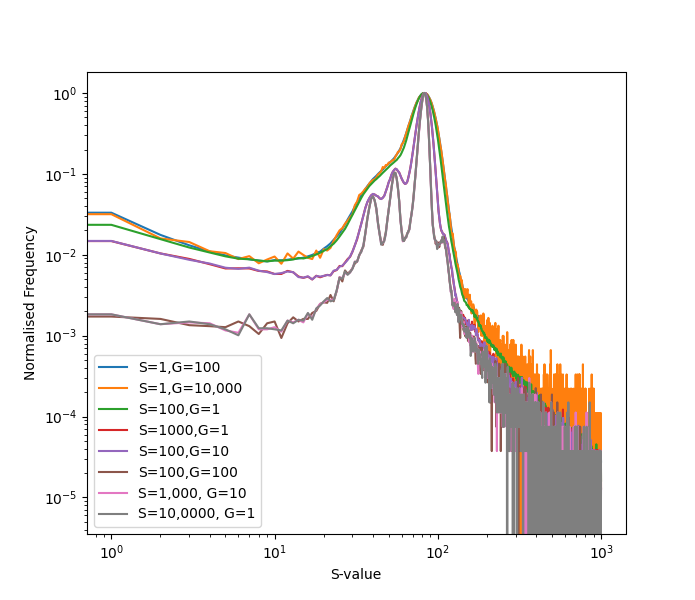
\includegraphics[width=\linewidth,keepaspectratio=true]{Figures/aggregate.png}
				\caption{The difference between the raw data and aggregated data for a cancer-bearing Tasmanian Devil genome (Devil-1545T2), demonstrating the prominence of the peaks at higher aggregate values ($S)$ and higher correlation-skipping ($G$). The $S$-value is equal to $\lfloor \frac{\sum_{i}^S k_{i\times G}}{S} \rfloor$, and hence equivalent (up to a binning) of the mean $k$ observed. The $y$ axis normalised such that the peak of every curve is at 1, for better comparison. Note that so long as $S > 100$, distributions with the same product $S\times G$ have the same pattern; indicating that we have achieved statistical independence.}\label{F:Aggregation}
			\end{figure}

			Fig. \ref{F:Aggregation} shows the distribution of $\lfloor\frac{s_i}{S}\rfloor$ for a variety of different values of $S$ and $G$. As expected, we see that when $ S> 100$, the structure of the distribution is independent of the product $SG$ (the $S=10,000, G=1$ curve is visually identical to the $S=100, G= 100$ one, for example) -- this demonstrates our earlier point, that increased summation is equivalent to omitting `correlated points' at high enough scales. However, the computational cost of computing our probability distributions is linear in the maximum observed value of $s_i$, which is itself a linear function of $S$. We would therefore prefer a lower value of $S$, which means a higher value of $G$ to achieve the same data-aggregation / amplification.
		}

		\subsection{Harmonic Fitting}
			\comment{
			% The primary problem with the na\"ive smoothing approach was that it (by definition) \textit{smoothed out} the data, in order that we might more easily spot \textit{discontinuities} in the data. These two points -- smoothing and discontinuities -- stand in direct opposition to each other, and so the method is inherently flawed.
			{The most obvious solution to denoise the Coverage Data is to simply pass a smoothing kernel over the data, potentially in combination with a binning algorithm, and use that to infer the underlying mean function that the data is oscillating around. Smoothing in this fashion serves as a generic way to extract a smooth curve from the extremely noisy data present, however it fails us on a number of grounds. Most importantly, this method can act to bias and manipulate the data in unforeseen and undesirable ways. Anecdotally, we found many occasions where the severity of an inferred deletion or duplication could be manipulated by altering the analysis lengthscale. }
			
			As a toy example, consider the (integer) sequence (1,5,1,1). If we we to pass a mean-kernel over this data, we would compute the mean to be $\bar{k}=2$, which is entirely unrepresentative of the composite parts.  A more involved statistical method is therefore required.
			
			The algorithm we shall present here is, in essence is a form of \textit{step detection}, a well known problem in signal processing. However, whilst there exist several out-of-the-box algorithms which might provide us with robust detections, we note that knowledge about the form of the data can be leveraged to provide a significantly more powerful and biologically meaningful inference. 
			}
			% \subsubsection{Model Assumptions}
			
			% 	We use the following knowledge and assertions as the underpinnings of our model.

			% 	Firstly, as argued in Appendix \ref{A:Theory}, we assume that the coverage, $k$, is distributed according to a (slightly modified) Negative Binomial probability mass function, which is characterised by the mean $\mu$ and variation $\sigma^2_\text{model} = \mu + \sigma^2$, where $\sigma^2 > 0$ is the variation associated with the biological variability.
	
			% 	% That is, $\mathcal{P}$ is the Negative Binomial distribution with mean equal to the mean of the error function, $\mu_\text{model} = \mu$, and the variance equal to $\sigma^2_\text{model} = \mu + \sigma^2$. We will use $\sigma$, rather than $\sigma_\text{model}$ throughout as it is independent of the mean and is only constrained to be positive, rather than $\sigma_\text{NB} > \mu$.
				
			% 	We assume that the mean $\mu$ is constant across a chromosome, except during gains or losses, where it changes discontinuously{, variations in sampling frequency (such as those induced by GC bias) are accounted for by the (generous) error rate of the probability model}. If we assume that the gains and losses we are identifying occur in all cells within the sample (i.e. no contamination or subclonality), then $\mu$ can only ever be integer multiples of the single-homolog coverage depth, $\nu$, such that $\mu = q \nu$, where $q$ is a non-negative integer equal to the multiplicity of the domain. We have a strong prior that most of the data should lie at $q = d_c$, the normal ploidy of the creature ($d$ can vary per chromosome, for example, the sex chromosomes, or in cases where the sample is known \textit{a priori} to be aneuploid).

			% 	We know that discontinuities must be separated by at least a distance $L$ on the linear genome, else they would have been resolved by the alignment tool. {However, we do not know where these lengths $L$ begin or end, so a 
			% 	strict binning is not sufficient.}

			
			% 	{The task of detecting the `steps', therefore, requires that we assign each base a value of $q$, the multiplicity (or `harmonic', in signal processing terms) of the base: gains and losses are trivially detectable wherever this integer value changes, in doing so we should ensure that our prior knowledge and model restrictions are obeyed. In Appendix \ref{A:Model} we produce a statistical model, \eref{E:Score} which permits us to assign a statistical score to a given set of proposed $\{q\}$ values for a genome.}

			% \subsubsection{Effects of Subclonality and Contamination}

			% 	Should the biological sample contain some cells which do not contain the same mutation - either as a function of subclonality in the mutation, or contamination of the sample with healthy cells\footnote{We shall term both mechanisms 'contamination', as they manifest similarly in the data} - we shall see a violation of one of our assumptions: the value of $\mu$ will not lie at integer multiples of $\nu$. When this effect is small, it does not meaningfully affect our analysis. At high degrees of contamination, however, it can blur the distinction between different values of $q$, and the classifier will struggle to reliably assign a harmonic since it will interpret the sample as lying halfway between two $q$ values -- something it is forbidden to include. 
				
				
			% 	{We model this behaviour (whilst retaining the power of the integer-assumption) by making a simplifying assumption:} that the degree of contamination is small and constant across the chromosome, and always tends to bias the coverage back towards the expected ploidy of the sample. If the degree of contamination is $\eta$, then we find that the expected 'contamination-biased frequency' is
			% 	\begin{spalign}
			% 		\mu^\prime_q & = \left[ (1-\eta)q + \eta d_c \right] \nu
			% 		\\
			% 		& = q^\prime\nu ~~~~~~~~\LLR~~~~~~~ q^\prime =  (1-\eta)q + \eta d_c
			% 	\end{spalign}
			% 	The effects of subclonality can therefore modelled by everywhere replacing $q$ with $q^\prime(q,\eta)$.


			% \subsection{The \codename{} Algorithm}
			% \begin{figure}
			% 	\begin{center}
			% 		\resizebox{!}{5cm}{ 
			% 		\begin{tikzpicture}
						
			% 			\node[anchor=east] at (-2,0) {Data:};
			% 			\draw (0,0)--++(3,0);
			% 			\node at (3.5,0) {\large ...};
			% 			\draw (4,0)--++(3,0);
			% 			\def\w{0.65}
			% 			\foreach \i in {1,...,3}
			% 			{
			% 				% \draw[fill=white] (\i-1,0) circle (0.35);
			% 				\draw[fill=white] ({\i-1-\w/2},{\w/2})--({\i-1+\w/2},{\w/2})--({\i-1+\w/2},{-\w/2})--({\i-1-\w/2},{-\w/2})--cycle;
			% 				\node at (\i-1,0) {$k_\i$};
			% 			}
						
						
			% 			\foreach \i in {1,...,2}
			% 			{
			% 				\draw[fill=white] ({\i+4-\w/2},{\w/2})--({\i+4+\w/2},{\w/2})--({\i+4+\w/2},{-\w/2})--({\i+4-\w/2},{-\w/2})--cycle;
			% 				\node at ({4+\i},0) {$k_{L+\i}$};
			% 			}
						
			% 			\def\fac{0.85}
						
			% 			\foreach \q in {0,...,4}
			% 			{
			% 				\def\y{\fac*\q+1}
			% 				\if\q2
			% 				\else
			% 					\draw[dashed,blue] (1,{2*\fac+1})--(6,\y);
			% 				\fi
			% 				\if\q1
			% 				\else
			% 				\draw[dotted,red] (0,{1*\fac+1})--(5,\y);
			% 				\fi
			% 				% \if\q4
			% 				% \else
			% 				% \draw[dashdotted,green] (0,{4*\fac+1})--(5,\y);
			% 				% \fi

			% 			}
			% 			\foreach \q in {0,...,4}
			% 			{
			% 				\def\y{\fac*\q+1}
			% 				\draw (-0.95,{2*\fac+1})--(-0.35,\y)--(2.75,\y);
			% 				\draw (4.25,\y)--(6,\y);
			% 				\node[anchor=east] at (-2,\y) {$q=\q$};
			% 				\foreach \i in {1,...,4}
			% 				{
			% 					\if\i4
			% 						\def\c{gray!10!white}
			% 						\draw[\c] (\i-1.5,\y)--++(2,0);
			% 						\draw[\c,fill=white] (\i-0.5,\y) circle (0.35);
			% 					\else
			% 						\draw[fill=white] (\i-1,\y) circle (0.35);
			% 						% \draw[fill=white] ({\i-1-\w/2},{\w/2})--({\i-1+\w/2},{\w/2})--({\i-1+\w/2},{-\w/2})--({\i-1-\w/2},{-\w/2})--cycle;
			% 						\node at (\i-1,\y) {\tiny $p_{\i\q}$};
			% 					\fi
								
			% 				}
			% 				\foreach \i in {1,...,3}
			% 				{
			% 					\if\i3
			% 						\def\c{gray!10!white}
			% 						\draw[\c] (\i+3,\y)--++(1,0)--(8,{2*\fac+1});
			% 						\draw[\c,fill=white] (\i+4,\y) circle (0.35);
			% 					\else
			% 						\draw[fill=white] (\i+4,\y) circle (0.35);
			% 						\node at (\i+4,\y) {\tiny $p_{L+\i,\q}$};
			% 					\fi
			% 					% \draw[fill=white] ({\i+4-\w/2},{\w/2})--({\i+4+\w/2},{\w/2})--({\i+4+\w/2},{-\w/2})--({\i+4-\w/2},{-\w/2})--cycle;
			% 					% \node at ({4+\i},0) {$k_{L+\i}$};
			% 				}
							
			% 			}
			% 			\draw[fill=white] (-1.25,{2*\fac+1}) circle (0.35);
			% 			\node at (-1.25,{2*\fac+1}) {Start};
			% 			\draw[fill=white] (8.25,{2*\fac+1}) circle (0.35);
			% 			\node at (8.25,{2*\fac+1}) {End};


						
			% 		\end{tikzpicture}
			% 		}
			% 		\caption{An example of a harmonic network -- only two sets of `jump edges' are shown (in red and blue) for clarity. In the full network, every node $p_{iq}$ is connected to $p_{i+1,q}$ and $p_{i+L,k\neq q}$. The graph is directional - vertices can only be traversed from left to right.}\label{F:Network}
			% 	\end{center}
			
			% \end{figure}

			% 	After determining the value of the free parameters (discussed in Appendix \ref{A:Parameters}), Equations \eqref{E:NormBin} and \eqref{E:Prior} provide everything we need to compute the score \eref{E:Score} for a proposed set of $\{q\}$. The task of detecting the most likely (subject to our priors) set of copy-numbers is therefore equivalent to identifying the set of $\{q\}$ which maximise \eref{E:Score}. This is an integer optimisation problem, with the limiting factor that the dimensionality of the solution is equal to the chromosome size.
			% 	% The Harmonic fitting method shows a vast improvement over the previous iteration - however it still suffers from a number of drawbacks, mostly associated with the somewhat dubious means by which the Bayesian tests were `bootstrapped' from each other (technically each successive probability should be fully conditioned on the previous set, rather than just stuffing that all into a simplistic prior).

			% 	% The Harmonic Network method is an attempt to a) make the assignment robust and mathematically sound and b) devise a method which is conceptually easier to understand and follow. 

			% 	Provided that we are able to make the assumption that there is some finite $Q$ such that $0 \leq q < Q$ across the entire genome, it is most convenient to think in terms of a \textit{network}, such that an assignment of $\{q\}$ corresponds to a unique path through the network: the optimal path is the one with the highest score.

			% 	The network is arranged in a series of layers (not dissimilar in appearance to the network diagrams of feedforward neural networks), each layer corresponding to a given base in the genome. The vertices (or `nodes') in the layer then correspond to different values of $q$ that might be assigned to that base. In short, a path which passes a node $n_{iq}$ corresponds to the $i^\text{th}$ base being assigned a harmonic of $q$.

			% 	The edges between vertices are directional, and obey the following rules, which are displayed graphically in Figure \ref{F:Network}:
			% 	\begin{enumerate}
			% 		\item The start node is connected to all nodes in the first layer, $n_{0,0\leq q < Q}$ 
			% 		\item The node $n_{i,q}$ is connected to nodes $n_{j>i}$ through \textit{step edges} and \textit{jump edges}
			% 		\begin{itemize}
			% 			\item Step Edges connect $n_{i,q} \to n_{i+1,q}$, i.e. the same harmonic in the next layer. Step edges have a cost equal to
			% 			\begin{equation}
			% 				\text{Cost}(n_{iq} \to n_{i+1,q}) = p_{\vec{\theta}}(k_{i+1} | q) + \begin{cases} 0 & q = d_c \\  \mathfrak{p}_\text{ploidy} & \text{else} \end{cases}
			% 			\end{equation}
			% 			That is, they incur a cost equal to the posterior probability that $k_{i+1}$ arises from the same $q$ as $k_i$, the $\mathfrak{p}_\text{ploidy}$ is the prior probability that the $q$ is equal to the normal ploidy.
			% 			\item Jump Edges connect $n_{i,q} \to n_{i+L,j\neq q}$, i.e. a different harmonic in a layer $L$ further along. This enforces the prior restriction that changes in $q$ must be above a certain length ($L$) in order to be considered valid. Jump Edges incur a cost equal to the posterior probability of assigning \textit{all} $k_{j}$ for $i < j \leq i + L$ to the new harmonic, and so the statistics must favour all of these $k$-values being assigned the same $q$ in order to consider a change in $q$ likely.
			% 			\begin{equation}
			% 				\text{Cost}(n_{iq} \to n_{i+L,j\neq q}) =\sum_{a = i+1}^{i+L} \left( p_{\vec{\theta}}(k_i | j) \right) +  \mathfrak{p}_\text{jump} + L \times  \begin{cases} 0 & j = d_c \\  \mathfrak{p}_\text{ploidy} & \text{else} \end{cases}
			% 			\end{equation}
			% 			We emphasise again that a path $n_{i,q} \to n_{i+L,j\neq q}$ means that $q_{i+1},....,q_{i+L}$ are all assigned the harmonic $j$, and that this is the only means by which a jump $q\to (j\neq q)$ is possible.
			% 		\end{itemize}
			% 		\item The nodes $n_{G-1,q}$ are connected to the End node
			% 	\end{enumerate}
				
			% 	Here we have used the shorthand $p_{\vec{\theta}}(k|q) = p(k| q^\prime\nu, \eta,\sigma,\gamma)$, our underlying distribution function given in \eref{E:NormBin}. From these rules it is a simple matter of using a basic shortest-path algorithm\footnote{{We are actually looking for the longest path, but minimising $|\mathcal{L}|$ is equal to maximising $\mathcal{L}$, so the distinction is trivial}}, using the associated cost of each node as the distance: step through each layer and compute the shortest path to each node in that layer, and then iterate until the end node is reached -- the longest path through this network corresponds to a unique $\{q\}$, which is then necessarily the one which maximises $\mathcal{L}$. An example of such a minimal path is shown in Fig. \ref{F:Path}.

				
				
			% 	The runtime of this algorithm scales as $\mathcal{O}(Q^2 G)$, where $Q$ is the maximum harmonic and $G$ is the number of bases being evaluated. However, if we naively construct this network in-memory it occupies a space $m Q G$, where $m$ is the memory footprint of an individual node. {A conservative estimate of the naive implementation gives the memory requirements (for a human genome) of $\approx$650GB, well beyond what most consumer devices are capable of. We note, however, that the network is only semi-local -- the network does not need any information more recent than the previous $L+1$ nodes, and so the network can be constructed on-the-fly. With $L=10^5$, this reduces the memory requirements to a mere $\approx 35$MB. }
				
			% 	% Assuming that $Q = 20$ and each node must know its score, $q$-value and a pointer to the previous node, this gives a conservative estimate of 646GB of active memory to construct a network for the entire human genome -- well beyond what most consumer devices are capable of. 

			% 	% However, we note that this network is `semi-local' -- by design, the edges never extend beyond a distance $L$ from the current base. By placing node node $n_{iq}$ at index $C_{i \% (L+1),q}$, we only need $LQ$ nodes in memory at once, rather than $GQ$, a drastic reduction in memory footprint: $L = 10^5$ reduces the memory footprint to only 34MB.

				

			% 	% However, we note that during the search for the value of $\nu$ (during which time many paths are evaluated, searching for the one which minimises $\mathcal{L}$), we only need the final `length' of the path, not the path itself. For the bulk of function calls to the path-tracing algorithm, therefore, we do not need to record the path - only its length -- and hence the runtime difference between the conveyor-belt algorithm and the naive algorithm is negligible, with the memory-footprint nevertheless vastly reduced.

			% 	\begin{figure}
			% 		\begin{center}
			% 			\resizebox{!}{7.3cm}{ 
			% 			\begin{tikzpicture}
							
			% 			%%network 
			% 				\node[anchor=east] at (-2,0) {Data:};
			% 				\draw (0,0)--++(7,0);
			% 				\def\w{0.65}
			% 				\foreach[count=\i] \j in {10,9,11,6,5,7,22,20}
			% 				{
			% 					% \draw[fill=white] (\i-1,0) circle (0.35);
			% 					\draw[fill=white] ({\i-1-\w/2},{\w/2})--({\i-1+\w/2},{\w/2})--({\i-1+\w/2},{-\w/2})--({\i-1-\w/2},{-\w/2})--cycle;
			% 					\node at (\i-1,0) {$\j$};
			% 				}
							
							
							
			% 				\def\fac{0.85}
			% 				\foreach \q in {0,...,4}
			% 				{
			% 					\def\y{\fac*\q+1}
			% 					\draw[black!30!white] (-0.95,{2*\fac+1})--(-0.35,\y)--(7.25,\y)--(8,{2*\fac+1});

			% 					\foreach \i in {0,...,5}
			% 					{
			% 						\foreach \qq in {0,...,4}
			% 						{
			% 							\if\q\qq

			% 							\else
			% 								\draw[black!30!white] (\i,{\q*\fac+1})--(\i+2,{\qq*\fac+1});
			% 							\fi
			% 						}
			% 					}
			% 				}

			% 				\draw[red,thick] (-0.95,{2*\fac+1})--(2.25,{2*\fac+1})--(3.75,{\fac+1})--(5,{\fac+1})--++(0.3,0)--(6.65,{4*\fac+1})--(7.25,{4*\fac+1})--(8,{2*\fac+1});
							
			% 				\foreach \q in {0,...,4}
			% 				{
			% 					\def\y{\fac*\q+1}
			% 					% \draw (4.25,\y)--(6,\y);
			% 					\node[anchor=east] at (-2,\y) {$q=\q$};
			% 					\foreach \i in {1,...,8}
			% 					{
									
			% 						\draw[fill=white] (\i-1,\y) circle (0.35);
			% 						% \draw[fill=white] ({\i-1-\w/2},{\w/2})--({\i-1+\w/2},{\w/2})--({\i-1+\w/2},{-\w/2})--({\i-1-\w/2},{-\w/2})--cycle;
			% 						\node at (\i-1,\y) {\tiny $p_{\i\q}$};
				
			% 					}
								
								
			% 				}
			% 				\draw[fill=white] (-1.25,{2*\fac+1}) circle (0.35);
			% 				\node at (-1.25,{2*\fac+1}) {Start};
			% 				\draw[fill=white] (8.25,{2*\fac+1}) circle (0.35);
			% 				\node at (8.25,{2*\fac+1}) {End};

			% 			%%plot
			% 				\begin{axis}[width=9.75cm,height=4cm,xlabel={Base Coordinate},ylabel={Coverage},at={(-0.5cm,-3cm)},scatter/classes={%
			% 					a={mark=o,fill=black}}]
			% 					\addplot[only marks,scatter src=explicit symbolic] table[row sep=crcr]{
			% 						x y label \\
			% 						1 10 a\\
			% 						2 10 a\\
			% 						3 11 a\\
			% 						4 6 a\\
			% 						5 5 a\\
			% 						6 7 a\\
			% 						7 22 a\\
			% 						8 20 a\\
			% 					};

			% 					\addplot[red] table[row sep=crcr]{
			% 						x y label \\
			% 						1 10 a\\
			% 						2 10 a\\
			% 						3 10 a\\
			% 						3.5 10 a\\
			% 						3.5 5 a\\
			% 						5 5 a\\
			% 						6 5 a\\
			% 						6.5 5 a\\
			% 						6.5 20 a\\
			% 						8 20 a\\
			% 					};
								
								
			% 				\end{axis}
			% 			\end{tikzpicture}
			% 			}
			% 			\caption{(Top panel) A demonstration of an optimal path through a network with $L=2$ and $\nu=5$, given some example coverage data. (Bottom panel) a projection of this path back onto the coverage distribution. For aesthetic reasons we have placed the transitions at half-integers -- in practice non-integer values of base index are meaningless.}\label{F:Path}
			% 		\end{center}
			% 	\end{figure}



			
				\bibliography{references.bib}
			\appendix
			{\small 
			\section{Mathematical Theory}\label{A:Theory}
				\subsection{Negative Binomial}
					The statistical model $\mathcal{P}$ for the coverage $k$, is derived from the common assumption that the genome is sampled via a Poisson distribution with mean $\lambda$, but where there are biological and experimental errors which change $\lambda$, such that the model is the convolution of a Poisson distribution, and some 'error distribution', which encodes the degree to which $\lambda$ varies. Maximal-entropy arguments imply that, barring any other knowledge, the Gamma distribution with mean $\mu > 0$ and variance $\sigma^2 > 0$ is the most general choice. 
					\begin{align}
						\mathcal{P} & = \int_0^\infty \gamma(\lambda| \mu,\sigma) \text{Poisson}(k|\lambda) \d \lambda
					\end{align}

					This integral is analytically computable, and results in the Negative Binomial, which has a well-known form:
					\begin{spalign}
						\text{NB}(k; r,p) & = \frac{\Gamma(k + r)}{k! \Gamma(r)} (1 - p)^k p^r
					\end{spalign}
	\comment{
					Here $\Gamma(x)$ is the usual Gamma function with the property $\Gamma(x+1) = x!$ when $x$ is a nonnegative integer. The resulting distribution is similar to the Poisson distribution, but `overdispersed', with a variance which is always greater than the equivalent Poisson's: $\sigma_\text{NB}^2 = \mu + \sigma^2$. The parameters $r$ and $p$ can be shown to be:
					\begin{spalign}
						r(\mu,\sigma) & = \frac{\mu^2}{\sigma^2}
						\\
						p(\mu,\sigma) & = \frac{\mu}{\mu + \sigma^2}
					\end{spalign}
					Where we emphasise again that $\sigma^2$ is the variance of the perturbation population, not of the Negative Binomial itself. As such, $\sigma^2$ is constrained only to be positive.

					

				\subsubsection{Sums of NB-Distributions}\label{A:Sums}
					As noted in the main text, however, we are not working with the raw coverage values, but instead with sums of coverage values; $s_i = \sum_j^S k_j$. Conveniently, the Negative Binomial also has the desirable property that it is additive \citep{RHBMaths}, which means that if $X \sim \text{NB}(r,p)$ and $Y \sim \text{NB}(s,p)$, then $X + Y \sim \text{NB}(r + s,p)$. That is, the sum of independent Negative Binomial variables is itself distributed according to a Negative Binomial. 

					If $k$ is distributed according to some $\text{NB}(r(\mu,\sigma), p(\mu,\sigma))$, then:
					
					\begin{equation}
						p(s | \mu, \sigma) = 	\text{NB}\left(s; S \times r(\mu,\sigma), p(\mu,\sigma)\right)
					\end{equation}

					The full distribution of $s$ can therefore be written as:
					\begin{equation}
						p(s| \mu,\sigma) = \frac{\Gamma(s + Sr)}{\Gamma(s+1) \Gamma(Sr)} (1 - p)^s p^{Sr}
					\end{equation}

					The key value of note for our purposes is that although this scales the mean of the distribution (predictably) by $S$, the standard deviation only scales as $\sqrt{S}$; the distribution therefore becomes more tightly peaked around the maximum. In the case where we are attempting to disentangle a distribution composed of multiple such overlapping distributions, this is a highly desirable property, as it will make the peaks more prominent. We see exactly this behaviour in Fig. \ref{F:Aggregation}.

					\subsubsection{Normalisation}

						Our methods require that our models be fully normalised (i.e. the probabilities sum to 1 over the non-infinite domain of interest). 
						
						We therefore ensure that each `harmonic' is individually normalised, defining the maximum value considered by our model as $M$:

						\begin{equation}
							B_s^q (\mu,\sigma^2) = \frac{\text{NB}(s | S\times r(\mu,\sigma), p(\mu,\sigma))}{\sum_{k=0}^M \text{NB}(k| S\times r(\mu,\sigma), p(\mu,\sigma))}
						\end{equation}

						This approach (instead of normalising the aggregate model) has the advantage of ensuring that the parameters $\epsilon$ and $w_q$ retain their intuitive meaning inside the domain of interest. 
				\subsection{Local Model}\label{A:Model}
					
					The fundamental assumption of our theoretical model is that there is always an integer number of copies of a sequence, with that integer varying as the copy number varies. Each segment of the genome therefore has a coverage distribution with a mean $q \nu$, where $q$ is the copy-number of that segment, and $\nu$ is some global mean, per-homolog coverage (in analogy to music, we term $\nu$ the `fundamental frequency', and $q$ values `harmonics').
					
					Our assertion is that, where large-scale insertions or deletions have occurred, $q$ changes discontinuously. The statistical problem therefore reduces to inferring what $q$ value the data has. 
					
					If we assume that the coverage is indeed distributed according to a Negative Binomial, then the probability of observing a coverage-sum $s$, given a known mean $\mu_q = q\nu$ and variance $\sigma^2$, error rate $\epsilon$ and error function $E(s)$ is simply:
					\begin{equation}
						p(s | q, \vec{\theta}) = \epsilon E(s) + (1 - \epsilon) B_s^q (\mu_q, \sigma^2) \label{E:MixtureModel}
					\end{equation} 
					Here $\vec{\theta}$ is compact notation for the parameters of the model: in this instance, $\vec{\theta} = (S,\nu,\sigma^2)$.
					\subsubsection{Contamination}

						A crucial inclusion in the model is a means to infer \textit{contamination}. Contamination in this sense is any confounding factor which means that $q$ is not a perfect integer. In the simplest possible case, the sample is contaminated by a fraction $\eta$ of normal somatic cells with copy number equal to the ploidy ($\mathcal{D}$); this would modify $q \to q + (\mathcal{D} - q) \eta$. The contamination value can then be provided or inferred directly.

						In practice we found that more complex cancers (especially those where the cancer modified the Ploidy) were fit poorly by this model. We therefore opted for a more flexible approach, providing `contamination parameters' for each harmonic:
						\begin{spalign}
							q^\prime & = q + \delta_q 
							\\
							\mu_q & = q^\prime \nu
						\end{spalign}
						
						
						% assumption that contamination will perturb the coverage back towards the normal ploidy of the sample, and that a fraction $\eta$ of the data is contaminated. This has the effect of modifying our statistics by the following:
						% \begin{spalign}
						% 	\mu_\text{contaminated} & = q^\prime\nu
						% 	\\
						% 	& = \left(q + (\mathcal{D} - q)\eta\right)\nu
						% \end{spalign}
						% When $\eta = 0$ it is clear that $\mu = q\nu$ as before, and when $\eta = 1$, then $\mu = d \nu$, i.e. the data is so contaminated that it looks like normal-ploidy. This can be made more complex by introducing a unique contamination factor for each $q$ (so $\eta \to \eta_q$), which may be necessary if it is believed that cancer subclonality is a bigger factor than noncancerous contamination. For our purposes, we leave it is a single constant.

						The contaminated model is therefore computed exactly as above, but replacing the Negative Binomial $r$ and $p$ parameters with:
						\begin{spalign}
							r_q & = \frac{\left(q + \delta_q\right)^2 \nu^2}{\sigma^2}
							\\
							p_q & = \frac{\left(q +  \delta_q\right)\nu}{\left(q + \delta_q\right)\nu + \sigma^2}\label{E:ContaminatedDist}
						\end{spalign}

						Although this model is more flexible, it loses the beneficial property that $\eta$ - the contamination fraction - is a biologically meaningful parameter. If possible (i.e. in the case of simple cancers) we would like to recover this property. We achieve this by imposing the following `contamination prior':
						\begin{spalign}
							\mathcal{C}(\{\delta_q\}, \eta) & = - \mathfrak{p}_\text{contamination} \sum_q \left( \delta_q - (\mathcal{D} - q) \eta\right)^2 \label{E:ContaminationPrior}
							% \\
							% \pdiv{\mathcal{C}}{\delta_q} & = -  2\mathfrak{p}_\text{contamination} \left( \delta_q - (\mathcal{D} - q) \eta\right)
							% \\
							% \pdiv{\mathcal{C}}{\eta} & =  2\mathfrak{p}_\text{contamination} \sum_q (\mathcal{D} - q) \left( \delta_q - (\mathcal{D} - q) \eta\right)
						\end{spalign}
						We retain an (approximate) estimate of the Contamination fraction; although it is now only a parameter which appears within the Prior.

					\subsubsection{The Error Function}

						The term $E(s)$ appears in \eref{E:MixtureModel} without further definition aside from being weighted to only contribute a fraction $\epsilon \ll 1$ to the total model. This is our \textit{Error Function}, and allows us to relax our assumption that only `perturbed Negative Binomials' contribute to the distribution. 

						For simplicity, we assume no functional form on the Error Function since it is, by definition, behaviour we have not modelled. We instead approximate this function with a piecewise-constant probability mass function with resolution $R_\epsilon$.

						\begin{equation}
							E(s) = \begin{cases}
								\mathcal{E}_0 & 0 \leq s < \Delta_0
								\\
								\mathcal{E}_1 & \Delta_0 \leq s < \Delta_0 + \Delta_1
								\\
								\vdots
								\\
								\mathcal{E}_{R_\epsilon -1} & M +1 - \Delta_{R_\epsilon -1} \leq s \leq M
							\end{cases}
						\end{equation}
						Where the width of each domain ($\Delta_i$) is given by:
						\begin{equation}
							\Delta_i = \begin{cases} 
							\left\lfloor \frac{M+1}{R_\epsilon} + \frac{1}{2} \right\rfloor & 0 \leq i < R_\epsilon -1
							\\
							M +1- \Delta_0 (R_\epsilon -1)& i = R_\epsilon -1
							\end{cases}
						\end{equation}
						A more compact notation can be constructed using the `window function', $\Omega(k)$:
						\begin{spalign}
							E(s) & = \mathcal{E}_{\Omega(s)}
							\\
							\Omega(s) & = \begin{cases}
								\left\lfloor \frac{s}{\Delta_0} \right\rfloor & s < M+1 - \Delta_{R_\epsilon -1}
								\\
								R_{\epsilon} -1 & \text{else}  
							\end{cases}
						\end{spalign}


						We assume that the Error Function is normalised by construction and therefore satisfied:
						\begin{equation}
							\sum_{s=0}^M E(s) = \sum_{i=0}^{R_\epsilon-1} \Delta_i \mathcal{E}_i = 1
						\end{equation}

						
					\subsubsection{Bayes' Theorem}

						For each base $i$, the probability of observing coverage-sum $s_i$, given that the current harmonic is $q$ is therefore $p(s_i | q, \vec{\theta})$. From Bayes' theorem, we can then invert this to find the probability $p(q | s_i, \vec{\theta})$; the probability that the harmonic is $q$ given that we have observed $s_i$.
						\begin{equation}
							p(q|s_i, \vec{\theta}) = \mathcal{N} {p(s_i | q, \vec{\theta}) \times \text{Prior}(q | \vec{\theta})}
						\end{equation}
						Here $\mathcal{N}$ is a multiplicative constant that depends only on the quality of the data (it is the `evidence'). The Prior is discussed in the next section; it is sufficient for now to note that it is in general non-separable and we must therefore consider the entire data in aggregate, rather than datapoint-by-datapoint. For a set of $n$ data points:
						\begin{equation}
							p( \{q\} | \{s_i\} , \vec{\theta}) = \mathcal{N}^n\left(\prod_i^n p(s_i | q, \vec{\theta}) \right) \text{Prior}(\{q\}| \vec{\theta})
						\end{equation}
						In logarithms:
						\begin{equation}
							\mathcal{L}(\{q\}) = \text{constant} + \text{LogPrior}(\{q\}) + \sum_i \log\big( p(s_i| q, \vec{\theta})\big) 
						\end{equation}

						The problem then reduces to optimising this function in order to maximise $\mathcal{L}$, and therefore find the most likely set of $\{q\}$ which describes our data.
						
					\subsubsection{The Prior}

						% The Prior 

						The \textit{Prior} is the function enumerating our beliefs about the structure of the output before we looked at the data. For the biological problem at hand, we know that our priors should be:

						\begin{enumerate}
							\item Consecutive values of $q_i$ should be similar
							\item $q_i$ cannot alternate values rapidly. Small-scale insertions and deletions would have been resolved by the aligner. 
							\item Most of the chromosome $c$ should be at $q_i = \mathcal{D}_c$ (equal to the ploidy)
						\end{enumerate}
					

					Therefore, we propose:
					\begin{spalign}
						\text{LogPrior}(\{q\})   = & \ln(\text{Prior}(\{q\}))
						\\
						= & \underbrace{\sum_i \varphi(q_i,\mathcal{D})}_{\text{ploidy}}  \mathfrak{p}_\text{ploidy}   + \underbrace{\sum_i \varphi(q_i, q_{i-1})  ~\mathfrak{p}_\text{change} }_{\text{similarity}}
						\\ 
						& ~+ \underbrace{\sum_{i=L} \sum_{j=i-L}^{i-1}\chi(q_j, q_{i-1})  ~\mathfrak{p}_{\infty} }_{\text{gap size}}
						\\
						\varphi(a,b)  = & (1-\delta_{ab}) = \begin{cases}
							0 & {a = b}
							\\
							1 & \text{else}
						\end{cases}\label{E:Prior}
					\end{spalign}
					The terms in the prior therefore act (in order), to penalise every base which is not at the expected diploid level by an amount $\mathfrak{p}_\text{ploidy}$, penalise every jump between dissimilar $q$ by an amount $\mathfrak{p}_\text{change}$ and to penalise jumps which occur within a distance $L$ of another jump by an amount $\mathfrak{p}_\infty$, which is a number $\approx -\infty$, but which has the property $0 \times \mathfrak{p}_\infty = 0$ -- rather than a penalty, this therefore acts as a \textit{forbiddance}, discarding models with such jumps.

					This final term of the prior -- the forbiddance -- is encoded in the structure of the algorithm (such models are never considered, rather than being considered and then removed). 

					The total prior also includes any other priors we have imposed; for example \eref{E:ContaminationPrior}:
					\begin{equation}
						\text{LogPrior}(\vec{\theta}) = \text{LogPrior}(\{q\}) + \mathcal{C}(\{\delta_q\}) 
					\end{equation}
				\subsection{Global Model}\label{A:Global}

					The `local' model discussed above is sufficient to infer the values of $q$ each base is to be assigned. However, it relies on a large number of  model parameters: the fundamental frequency $\nu$, the variance $\sigma^2$, the contamination s$\{\delta_q\}$, the error rate $\epsilon$ and the components of the residual function $E(s)$. Before we can assign $\{q\}$ we must infer these values. We could place them into the same inference routine as $\{q\}$, except that this requires genome-scale computations, and so rapid iteration and optimisation is not feasible. 

					Instead, we aggregate the data into a histogram; rather than worrying about \textit{where} each $q$ is, we instead attempt to compute \textit{how many there are}.

					Taking our data $D = \{s_1, s_2, ...\}$, we transform it into a vector $\vec{N}$ such that $N_r$ is the number of times that $s = r$ occurs in the data. For convenience, we also truncate the data at some maximum value, $M$. This prevents wasting computation time on extreme outliers. $M$ can usually be selected by ensuring that 99\% of the data lies below the value.

					The Global Model differs from the Local Model insofar as, rather than trying to compute where two populations are separated, we model the genome as a mixture model of all the harmonics given in \eref{E:ContaminatedDist}:
					\begin{spalign}
						p_\text{global}(s|\vec{\theta}) & = \sum_{q=0}^Q w_q p(s|q,\vec{\theta}) 
						\\
						& = \epsilon E(s) + (1-\epsilon) \sum_{q=0}^Q w_q B_s^q \label{E:DefinePGlobal}
					\end{spalign}
					Here $w_q$ are the weights of each harmonic in the mixture model; these are (approximately) equal to the fraction of the genome assigned to each $q$. However, unlike in the local model, we have no idea \textit{where} those $q$ values are. The $w_q$ are interpreted as probabilities (i.e. the probability of belonging to members of the mixture), and thus are constrained such that $w_q \geq 0$ and $\sum_q w_q = 1$.

					If this condition on $w_q$ holds, and both $E(s)$ and $B_s^q$ are independently normalised on the domain $[0,M]$, it is also guaranteed that $\sum_s p_s = 1$. With this normalisation, we can use Bayes' theorem to set up a likelihood:
					\begin{equation}
						\mathcal{L}_\text{global}(\vec{\theta}) = \sum_{s=0}^M N_s \log\left({p}_s(\vec{\theta})\right) + \text{LogPrior}(\vec{\theta})
					\end{equation}
					
					This then has the property that:
					\begin{equation}
						\pdiv{\mathcal{L}_\text{global}}{\vec{\theta}} = \sum_s^M \frac{N_s}{{p}_s}  \pdiv{p_\text{global}(s,\vec{\theta})}{\vec{\theta}} + \pdiv{\text{LogPrior}}{\vec{\theta}}\label{E:MainDerivative}
					\end{equation}
					
			
				\subsubsection{The Derivatives}

					With \eref{E:MainDerivative}, it is clear that when optimising $\mathcal{L}_\text{global}$ (and hence determining the parameters for the local model), we need to be able to compute the derivatives of $p_\text{global}$ (\eref{E:DefinePGlobal}) with respect to the model parameters. This is not a particularly conceptually challenging task, but due to the number of components of the model, it can get rather convoluted.
				
					We begin with introducing a number of auxiliary variables. These enable us to perform an unconstrained optimisation, whilst ensuring the constraints of our parameters are met:
					\begin{alignat}{2}
						\nu & = \exp(x) \quad && \text{Frequency always positive}
						\\
						\sigma^2 &= \exp(y) \quad && \text{Variance always positive}
						\\
						w_q & = \frac{\exp(z_q)}{\sum_r \exp(z_r)}\quad && \text{$w_q$ always positive and sum to 1}
						\\
						\epsilon & = \frac{e}{1+\exp(-\phi)} && \text{Error rate always between 0 and $e$}
						\\
						\mathcal{E}_i & = \frac{\exp{(\rho_i)}}{\sum_{j=0}^{R_\epsilon-1} \Delta_j \exp{(\rho_j)}} && \text{Error function normalised on $[0,M]$}
						\\
						\delta_q & = d_- + \frac{d_+ - d_-}{1 + \exp(-\psi_q)} ~~&& \text{Contamination always between $d_-$ and $d_+$}
						% \eta & = \frac{h}{1 + \exp(-\psi)} && \text{Contamination rate always between 0 and $h$}
						% & q && m && n
					\end{alignat}
					We then define the following intermediary values:
					\begin{spalign}
						% \pdiv{B_s^q}{p_q} & = B_s^q \left(\frac{\langle s_q \rangle - s}{(1-p_q)}\right)
						% \\
						% \pdiv{B_s^q}{r_q} & = B_s^q S \left(\digamma(s + Sr_q) - \langle \digamma_q \rangle \right) = B_s^q S \gamma_s^q
						% \\
						\langle s \rangle_s & = \sum_s s B_s^q
						\\
						\langle \digamma \rangle_q & = \sum_s B_s^q \digamma(s + S r_q)
						\\
						\tau_s^q & = S r_q \left(\digamma(s + Sr_q) - \langle \digamma_q \rangle \right)
						\\
						\lambda_s^q & = p_q \left( \langle s_q \rangle - s\right)
					\end{spalign}
					Where $\digamma(x)$ is the (first-order) digamma function. This allows us to write the various derivatives as:
					\begin{description}
							
						% \item[\textbf{$q^\text{th}$ Mean}]
						% \begin{spalign}
						% 	\pdiv{p_\text{global}(s)}{\mu_q} & =  (1-\epsilon) w_q \left( \frac{2 r_q}{\mu_q} \pdiv{B_s^q}{r_q}  + \frac{p_q(1-p_q)}{mu_q} \pdiv{B_s^q}{p_q}\right) 
						% 	\\
						% 	& = \frac{(1-\epsilon)}{\mu_q} w_q B_s^q \left( 2 S r_q \gamma_s^q  + p_q \left(\mu_q S - s\right)\right) 
						% \end{spalign}
						\item[\textbf{Fundamental Frequency}]
						\begin{spalign}
							\pdiv{p_\text{global}(s)}{x} & = (1-\epsilon) \sum_q w_q B_s^q \left( 2 \tau_s^q + \lambda_s^q\right) 
						\end{spalign}
						\item[\textbf{Variance}]
						\begin{spalign}
							\pdiv{p_\text{global}(s)}{y} & = - (1-\epsilon) \sum_q w_q B_s^q \left( \tau_s^q + \lambda_s^q \right) 
						\end{spalign}
						\item[\textbf{Weights}] \begin{spalign}
							\pdiv{p_\text{global}(s)}{z_q} & = w_q \left(B_s^q - \sum_r w_r B_r^q \right)
						\end{spalign}
						\item[\textbf{Contamination}]
						\begin{spalign}
							\pdiv{p_\text{global}(s)}{\psi_q} & 
							= (1-\epsilon)w_q B_s^q \left( 2\tau_s^q + \lambda_s^q \right) 
							\\ & \times \frac{(\delta_q - d_-)(d_+ - \delta_q)}{(d_+ - d_-)(q + \delta_q)}
							% = (1-\epsilon) \eta(1 - \frac{\eta}{h})\sum_q &\left[ w_q B_s^q \left( 2 S r_q \gamma_s^q  + p_q \left(\mu_q S - s\right)\right) \frac{(\mathcal{D} - q)}{q + (\mathcal{D} - q)\eta} \right]
						\end{spalign}
						\item[\textbf{Error Rate}]  \begin{spalign}
							\pdiv{p_\text{global}(s)}{\phi} & = \epsilon \left(1 - \frac{\epsilon}{e} \right) \left( E(s) - \sum_q^Q w_qB_s^q\right)
						\end{spalign}
						\item[\textbf{Error Function}]
						\begin{spalign}
							\pdiv{p_\text{global}(s)}{\rho_j} = \epsilon \mathcal{E}_{\Omega(s)} \left( \delta_{j,\Omega(s)} - \mathcal{E}_j \Delta_j\right)
						\end{spalign}
						(Note here that we are using $\delta_{a,b}$ in the sense of the Kroencker Delta, not the contamination parameter, $\delta_q$)
					\end{description}

			
			}




			\section{GenCHORD Algorithm}\label{A:Algorithm}

				\subsection{Parameter Estimation}\label{A:Inference}

				\subsection{Gamma-Digamma Simplification}

					The nature of the Negative Binomial requires that we be able to compute the following (transcendental) functions of the Gamma function ($\Gamma$) and its derivative ($\digamma$):
					\begin{spalign}
						f(s) & =  \log\left(\frac{\Gamma(s + r)}{\Gamma(r)}\right) 
						\\
						h(s) & =  \digamma(s + r) - \digamma(r)
					\end{spalign}
					There exist efficient methods to approximate these functions (for example, the C++ standard \citep{CPPStandard} guarantees the existence of \verb|std::lgamma| to compute $\log(\Gamma(x))$). 

					Our uses, however, require being able to compute these functions for all values of $s$, sequentially, on the domain $[0,M]$. This is a considerable source of computational expenditure, and can be vastly reduced by the use of the following identities, leveraging our knowledge that $s \in \mathbb{N}$ and $r > 0$:
					\begin{spalign}
						f(s) &= \begin{cases} 0 & s = 0
							\\
							f(s-1) + \log(s-1+r) & \text{else} \end{cases}
						\\
						h(s) & = \begin{cases} 0 & s = 0
							\\
							h(s-1) + \frac{1}{s - 1 + r} & \text{else} \end{cases}
					\end{spalign}
					Although slower for computing \textit{individual} values of $h(s)$ and $f(s)$, this recurrence relation allows us to compute \textit{sequential} values with vastly reduced overhead: replacing expensive $\Gamma$ and $\digamma$ calls with (comparatively) cheap division and logarithms. This can result in speedups in excess of 10x when $S$ is large.


				% The Gamma function ($\Gamma$) and its derivative, the digamma function ($\digamma$) are transcendental and relatively costly to compute. However, since $s \in \mathbb{N}$ and $r > 0$ by definition, we can use an alternative representation: 
				% \begin{spalign}
				% 	f(s) = \log\left(\frac{\Gamma(s + r)}{\Gamma(r)}\right) & = 
				% \end{spalign}
				% For individual computations, this method is vastly slower than the common (and often inbuilt) methods for approximation, especially when $s$ grows large.

				% Our uses, however, require being able to compute these functions for all values of $s$, sequentially, on the domain $[0,M]$, in which case we can convert these into a recurrence relation:
				% \begin{spalign}
				% 	a
				% \end{spalign}
				
				% each call to $\Gamma$ is replaced by a logarithm and an addition, whilst $\digamma$ is replaced by a division and an addition.
			}
\end{document}